\chapter{Burlesque}

\section{logaritmo ellittico}
Lo scopo di questa chiacchera è dare una idea di come si possa {\it invertire} la funzione $\wp: \bbC/L \rar \widetilde{E}$, o meglio costruirne delle determinazioni.\\
L' analogia con le quadriche $x^2+y^2=1$ e la funzione $\sin$ è forte: stiamo cercando l' equivalente del logaritmo complesso.\\
Accettiamo il fatto che si possa dare una nozione di forma differenziale sulla cubica (che in fondo è una onesta varietà). Allora definiamo una forma differenziale $\omega$ su $\widetilde{E}$ dandone l' espressione in coordinate locali $(x,y)$:
$$
\omega=\frac{dx}{y(x)}=\frac{dx}{\pm\sqrt{ax^3+bx+c}}
$$
questa forma è definita su $\bbC\setminus\{\alpha, \beta, \gamma\}$ le tre radici della cubica ma ha un problema di scelta della determinazione della radice; perchè sia ben definita occorre operare dei {\it tagli} $\gamma_1$ e $\gamma_2$ che collegano le radici $\alpha,\beta$ e $\gamma,\infty$. Se rimuoviamo questi cammmini dal nostro piano una scelta del segno nella forma $\omega$ è coerente ovunque e si può felicemente integrare. Inolre aver tolto l' $\infty$ ci permette di passare dal piano complesso alla sfera di Riemann.\\
Alla fine abbiamo due forme $\omega_+$ ed $\omega_-$ definite su $\widehat{\bbC}\setminus\{\gamma_1,\gamma_2\}$. Adesso avviene il passaggio critico: dobbiamo incollare queste due sfere tramite l' identificazione rispettiva dei cammini che abbiamo rimosso:
$$
\gamma_1^+\sim \gamma_1^-\ \ , \ \ \gamma_2^+\sim\gamma_2^-;
$$
quest' incollamente a priori è topologico ma può essere fatto in modo da mantenere la struttura complessa, e questo è non ovvio. però dato che topologicamente il risultato è un toro la struttura complessa su di lui, per il teorema di classificazione di Riemann, deve essere quella standard.\\
Questo toro che abbiamo trovato è naturalmente quello corrispondente alla nostra cubica, anche se neanche questo sembra ovvio.\\
Le nostre forme differenziali nell' incollamento non si perdono, anzi si uniscono coerentemente dando luogo quindi ad una unica $\Omega$ definita sul toro.\\
Questa forma agisce naturalmente, tramite integrazione, sui cammini sul toro, o meglio sulle loro classi di equivalenza omotopica, o meglio sull' abelianizzato del gruppo fondamentale:
$$
\int_{c_1 * c_2} \Omega=\int_{c_2 * c_1} \Omega
$$
Insomma abbiamo costruito l' integrale sulle classi di omologia del toro (che ha primo gruppo di omotopia/omologia $\bbZ\times \bbZ $), fissati due generatori $\{c_1,c_2\}$ si ha:
$$
\int: \bbZ\times \bbZ \rar \bbC \ \ \ \ \ (m_1,m_2)\mapsto m_1 \int_{c_1} \Omega+m_2 \int_{c_2} \Omega
$$
L' immagine di questa mappa, per delle ragioni da chiarire, dovrebbe proprio essere il reticolo $L$ soggiacente al toro.\\
Si arriva quindi alla definizione di logaritmo ellittico, fissato $O\in \widetilde{E}$:
$$
\widetilde{E}\rar \bbC/L\ \ \ \ P\mapsto \int_O^P \Omega
$$
questi ultimi passaggi esulano persistentemente dalla mia comprensione.
\section{mappe tra curve ellittiche diverse}
Avevamo visto che una mappa olomorfa tra due tori $T_1$ e $T_2$, a meno di traslazioni, era per forza moltiplicativa. La domanda che ci poniamo è come questa mappa si legga a livello di cubiche: può essere una funzione trascendente?
\begin{proposizione}
Se $T_1$ e $T_2$ sono tori, $\widetilde{E}_1$ e $\widetilde{E}_2$ le corrispondenti cubiche, $\mu$ complesso non nullo; allora la mappa $\phi_\mu:\widetilde{E}_1\rar\widetilde{E}_2$, indotta dalla moltiplicazione per $\mu$ sui tori, è una funzione razionale delle coordinate.
\end{proposizione}
\begin{proof}
Sappiamo che, se i tori sono indotti da reticoli $L_1$ ed $L_2$, vale:
$$
\mu L_1\subseteq L_2;
$$
utilizzando le funzioni di Weierstrass abbiamo le parametrizzazioni (usiamo carte affini sulla cubica):
$$
\wp_i:T_i\rar \widetilde{E}_i \qquad \ \ z \mapsto (\wp_i(z),\wp_i'(z))\ \ \ \ i=1,2
$$
quindi possiamo scrivere la relazione di commutazione nel modo più efficiente:
$$
\phi_\mu(\wp_1(z),\wp_1'(z))=(\wp_2(\mu z),\wp_2'(\mu z))
$$
a questo punto osserviamo che, grazie alla condizione $\mu L_1\subseteq L_2$, la funzione $\wp_2(\mu z)$ (e la sua derivata) è periodica anche per $L_1$ e dunque appartiene a $\bbC(\wp_1,\wp_1')$; questo implica che la funzione $\phi_\mu$ sia razionale.
\end{proof}
A questo punto è obbligatorio un esempio di reticoli che abbiano morfismi in sè stessi non dati da moltiplicazione per interi:
\begin{fatto}
Per $L=\bbZ[i]$ la corrispondente cubica è $y^2=x^3-x$ e un' isogenia qui è data da $(x,y)\mapsto (-x,iy)$.
\end{fatto}
\section{Grado di una funzione razionale su una curva ellittica}
Diamo la definizione di grado.
\begin{definizione}
Consideriamo una mappa $f:\widetilde{E}\rar\ \bbC$ che sia funzione razionale delle coordinate. Una tale $f$ verrà detta {\it funzione razionale}. Se è noncostante il suo grado è definito come:
$$
\deg(f,\alpha)=\#\{x\in \widetilde{E}:f(x)=\alpha\}
$$
dove $\alpha$ è un qualsiasi valore regolare di $f$.
\end{definizione}
Il fatto vero e a priori non ovvio è che questo numero sia finito e non dipenda da $\alpha$.\\
Osserviamo subito che per il T2 sulle funzioni ellittiche $f$ ed $f-\alpha$ hanno stesso numero di poli (ovvero di zeri) e quindi:
$$
\deg(f,\alpha)=\#\{f=\alpha\}=\#\{f-\alpha=0\}=\#\{\mbox{poli di } f-\alpha\}=\#\{\mbox{poli di } f\}
$$
e abbiamo eliminato la dipendenza da $\alpha$.\\
Il legame tra grado e curve ellittiche è dato dal seguente
\begin{esercizio}
Sia $f$ funzione ellittica non costante, allora vale:
$$
\deg f= [\bbC(\wp(z),\wp'(z)):\bbC(f(z))].
$$
\end{esercizio}
Con questa sfida si chiude, a Dio piacendo, la lezione di Umberto.



\section{Biliardi ellittici}
\newthought{Introduciamo un altro modo} in cui si ottengono le curve
ellittiche dalle ellissi \notamargine{Abbiamo infatti già visto che si
  possono ottenere come integrali della lunghezza d'arco di un'ellisse}.

Prendiamo un'ellisse di equazione $ax^2 + by^2 = 1$ e supponiamo di
giocare a biliardo sull'ellisse: facendo partire la pallina da un punto
la lanciamo contro il bordo dell'ellisse su cui rimbalza secondo la nota
legge della riflessione \notamargine{Ovvero rispetto alla tangente
  all'ellisse nel punto rimbalza via con lo stesso angolo, come indicato
  in figura}

\begin{center}
  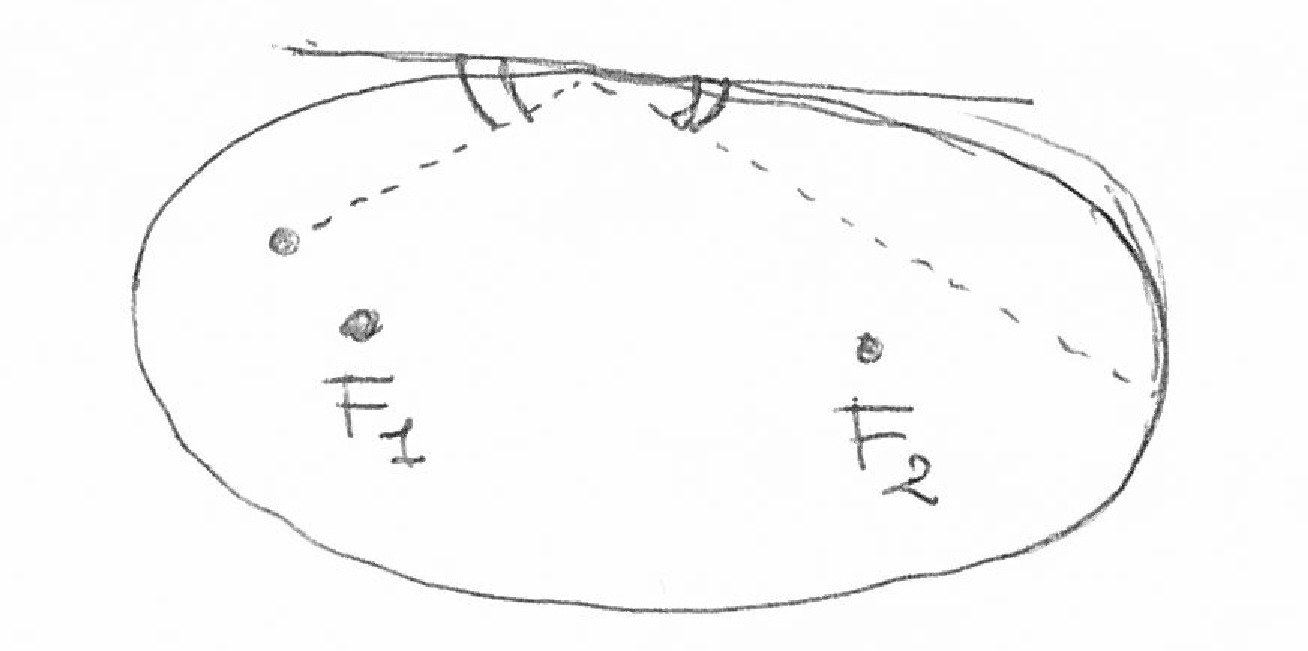
\includegraphics[width=8cm]{lezione-170123-fig1}
\end{center}

Una cosa che è nota da tempo è che le rette che compongono la
traiettoria sono tutte tangenti ad un'altra ellisse ``caustica'' che ha
gli stessi fuochi della prima: abbiamo quindi una famiglia ad un
parametro di ellissi che descrive tutte le possibili traiettorie.

\newthought{Vediamo allora che succede} quando prendiamo un punto $P$
sul bordo dell'ellisse ed una retta $l$ con $P \in l$ e tangente alla
caustica:

Possiamo definire un'applicazione $\phi$ dalle coppie punto-retta in sè
che è la funzione di ``evoluzione'' della traiettoria sul biliardo,
ovvero manda la coppia $(P, l)$ in $(P', l')$ con $P'$ l'altro punto di
intersezione della retta $l$ con l'ellisse e $l'$ la retta passante per
$P'$ che segue la legge della riflessione con $l$.

\notamargine{
  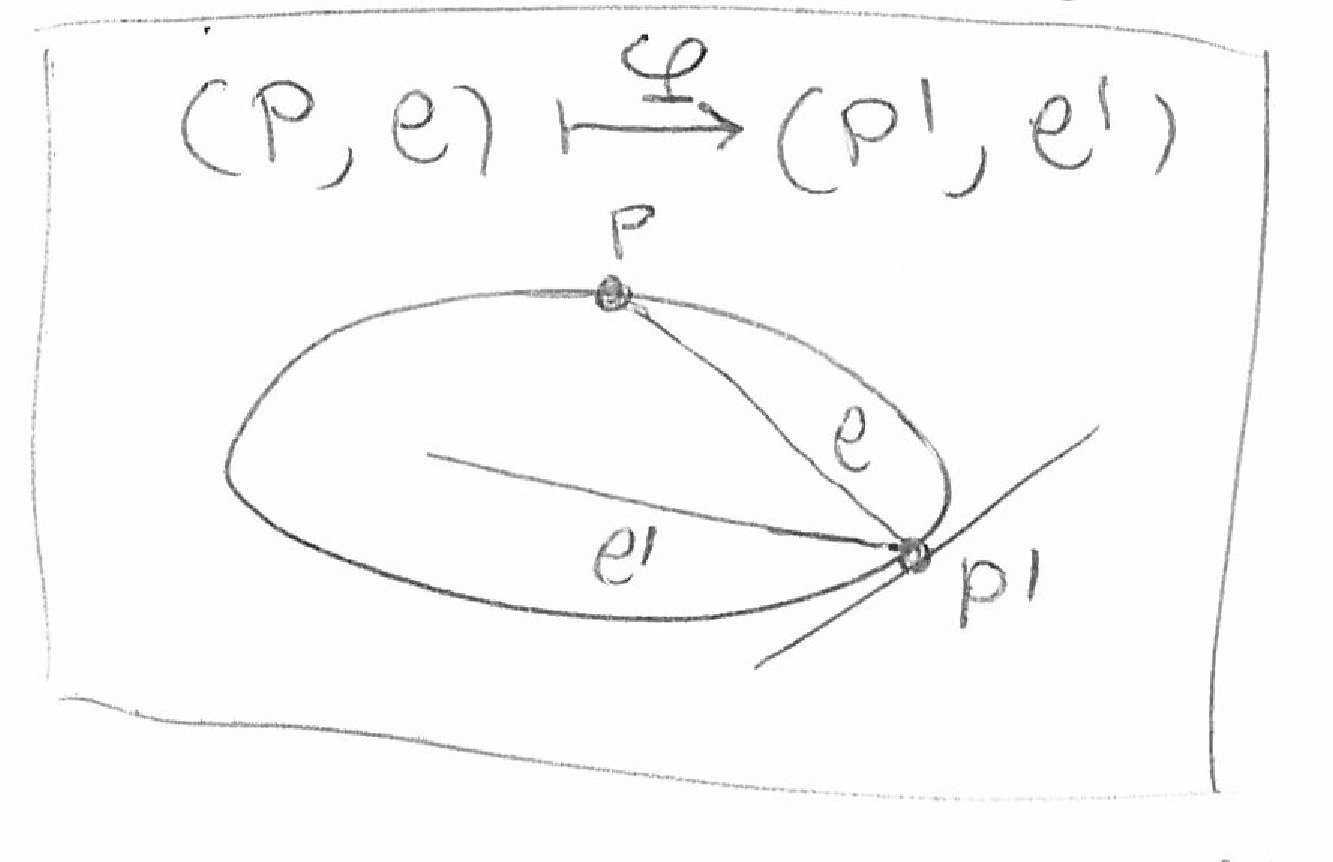
\includegraphics[width=4cm]{lezione-170123-fig2}
}

\newthought{È noto} che le tangenti in $\bbP^2$ ad una conica sono
parametrizzate da un'altra conica: la conica duale.
\notamargine{Tutto ciò non è difficile da verificare: se la conica $\cC$
  ha equazione $f = ax^2 + by^2 + cz^2$ e $(x_0, y_0, z_0) = P \in \cC$
  allora $(\nabla f)_P = (2ax_0, 2by_0, 2cz_0)$ e, ricordando che tutti
  i punti/vettori considerati sono in $\bbP^2$ si ha che dare la retta
  tangente in $P$ è uguale a fornire il vettore $(\nabla f)_P$. D'altra
  parte si riesce ovviamente a recuperare il punto $P$ dato $(\nabla
  f)_P$ a cui è tangente (basta vedere la formula scritta sopra in
  coordinate, visto che i coefficienti della conica sono noti)}
Allora il luogo di punti su cui la $\phi$ agisce è una sottovarietà
(algebrica) di $C_1 \times \hat{C_2}$, con $C_1 = \text{punti della
  conica}$ e $\hat{C_2} = \text{conica duale delle rette tangenti}$.

Il luogo di punti è dato dalle coppie $(P, l) \in C_1 \times \hat{C_2}$
tali che $P \in l$ (che è una condizione chiusa, ovvero dà luogo ad una
sottovarietà algebrica). Questa è anche una superficie di Riemann.

Scrivendo l'equazione si ottiene una curva ellittica e l'operazione
$\phi$ si rivela essere una traslazione sulla cubica detta ``gioco di
Poncelèt''.

Il gioco ``finisce'' se e solo se la traslazione $\phi(x) = x + \tau$ ha
un punto di ordine finito, ovvero $\exists n$
$\phi^n (x) = x + n\tau = x$ se e solo se $n\tau \in L$, il
reticolo. Ovvero si avrebbe $\phi^n(x) = x$ per ogni punto. Allora se il
gioco finisce per una traiettoria finisce per tutte le altre, cosa che
non è per nulla banale.

\notamargine{Come curiosità, se il gioco non finisce, le traiettorie del
  biliardo sono dense nello spazio tra le due ellissi}
